\documentclass[mathserif]{beamer}

\usetheme{UB}
\graphicspath{{figs/}}

\date{September 3, 2014}
\author{Paul T. Bauman}
\institute{Department of Mechanical and Aerospace Engineering\\
Computational and Data-Enabled Science and Engineering\\
University at Buffalo, State University of New York}
\title[Statistics for Complex Multiphysics]{Statistical Methods for Complex Multiphysics Problems}

\begin{document}

%===============================================================================
% Title Slide
%===============================================================================
\begin{frame}
\titlepage
\end{frame}

%===============================================================================
% Title Slide
%===============================================================================
\begin{frame}
\frametitle{Slide Title}

% Block with title
\begin{block}{Block Title}
\begin{itemize}
\item Stuff 1
\item Stuff 2
\end{itemize}
\end{block}

% Block without title
\begin{block}{}
\begin{itemize}
\item Stuff 3
\end{itemize}
\end{block}

\begin{equation}
f(x) = x^2
\end{equation}

\end{frame}


%===============================================================================
% Title Slide
%===============================================================================
\begin{frame}
\frametitle{Two Column Slide w/ Picture}

\begin{columns}
\begin{column}{0.45\textwidth}
\begin{block}{}
\begin{itemize}
\item All image files go in the rawfigs directory
\item The Makefile will figure out what to do with them
\item Prefer scalable vector .pdf files and .eps or .png files
\end{itemize}
\end{block}
\end{column}
%
\begin{column}{0.45\textwidth}
\begin{block}{Fancy Picture}
\centerline{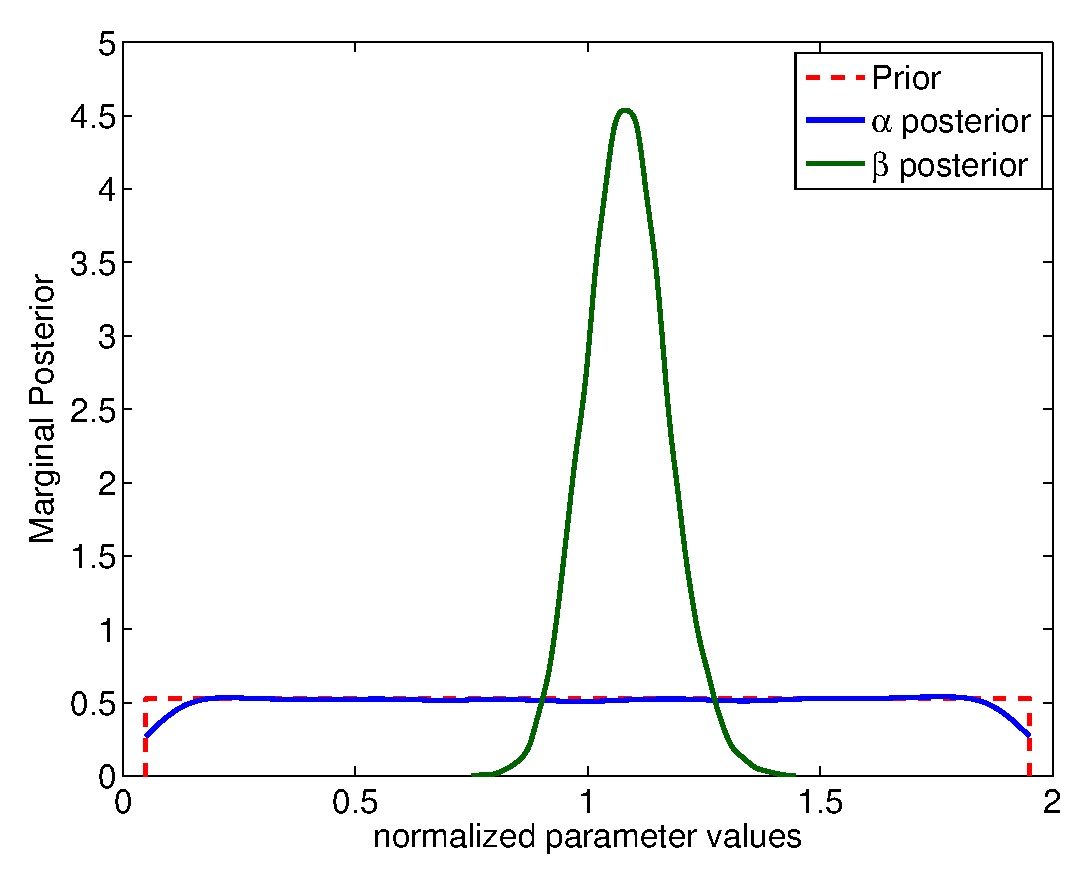
\includegraphics[width=\linewidth]{alpha_beta_synthetic_post}}
\end{block}
\end{column}
\end{columns}

\end{frame}

\end{document}
